\chapter{Dynamic Pipeline Framework in Haskell}\label{dp-hs}
One of the fundamental piece of the present work as we have described in ~\autoref{intro} and ~\autoref{prelim},
is the design and implementation of \acrfull{dpfh}: a \acrshort{dpf} written in \acrshort{hs} which allow \acrshort{hs} users
to implement any suitable algorithm in \acrshort{dp}, providing the correct abstractions that helps on that matter.

During the process of conducting this research, we implemented \acrshort{dpfh}~\cite{dynamic-pipeline} and published into 
Hackage (The public Haskell Package Repository of Libraries).
In this chapter we are going to describe the design and implementation details of \acrshort{dpfh}.

\section{Framework Model}

\subsection{Background}
Any suitable library or framework should provide the user the right level of abstraction that removes and hides enough complexity, 
to allow the developer to focus on the problem that it needs to solve.
There are several design approximation to implement a library or framework: \emph{configuration based} where the user only 
focus on follows specific configuration files and provides the runtime system of the framework those configurations to execute the program,
\emph{convention over configuration approach} where the user writes his code and definition following certain pattern in naming or source disposition 
and the framework figures out what needs to be generated on that matter, \emph{functionality based} where the framework or library provides certain amount
of functionality implemented and the user needs to compose those functions to achieve its results and finally \emph{domain specific language models} where 
the framework or library provides a new language that represents the abstraction that we need to deal with. 

In the \emph{domain specific language} approach~\cite{dsl} there exists two types of abstraction: \acrfull{dsl} and \acrfull{edsl}. \acrshort{dsl} or 
usually called external \acrshort{dsl} the propose is to create a completely new language with each own semantic, syntax and interpreter. These are not 
Turing-Complete languages~\cite{turing-comp} because its scope is domain specific as the name indicates. On the other hand \acrshort{edsl} are syntactically 
embedded in the host language of the library, the user writes in the host language library but using the abstractions provided by it with strong checking of 
the constrains imposed by this embedded language.

\acrshort{dpfh} follows a \acrshort{edsl} approach taking advantage of the strong type \acrshort{hs} system giving the user correctness proof at type-level.

\subsection{Framework Design}
In this section we are going to focus on the design of the \acrshort{dpfh} using a \acrshort{edsl} approach. We have built a framework that contains
three important components: \acrshort{dsl}, \acrshort{idl} and \acrshort{rs}. 

\begin{figure}[!ht]
  \centering
  \begin{minipage}{\textwidth}
   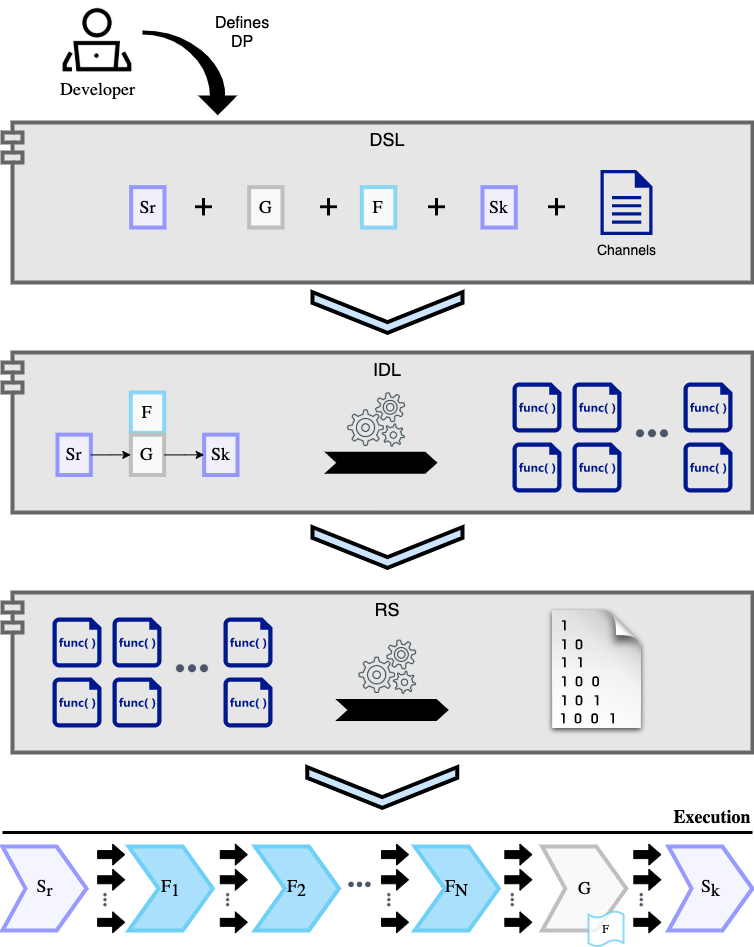
\includegraphics[width=1\textwidth, height=0.6\textheight]{dpf_haskell_v3.png}
    \caption{Architectural view of \acrshort{dpfh}}
    \label{fig:dpfh:1}
  \end{minipage}
\end{figure}

In \autoref{fig:dpfh:1} we can appreciate the different components mentioned before that are the grey boxes.

\paragraph{DSL} The user interacts with the \acrshort{dsl} component where defines how the \acrshort{dp} disposition
should be and what are the channels that are going to communicate the different stages of the pipeline: for example in the
case of \autoref{prole} that we develop the \acrshort{wcc} algorithm, the user knows that is going to received from the Input 
the edges of the graph and it needs two channels between $\iwcc$, $\gwcc$ and $\owcc$, one for sending the edges and another for sending
the accumulated connected components. 

\paragraph{IDL} The user interacts with the \acrshort{idl} which guide him to build the functions with the algorithms needed for each stage: 
$\iwcc$, $\gwcc$, $\owcc$, $\fwcc$ and actors. Based on the definition provided in the \acrshort{dsl}, the framework will indicate the user 
how that definition is interpreted in the context of \acrshort{dp} and what functions should provide.

\paragraph{RS} Once we have the \acrshort{dp} definition and the functions provided by the user with the algorithm solution, the framework
can be fed with this components to execute the program. 

\section{Implementation}
In this section we are going to describe the details of all the techniques used for implementing each of the components described before.


\section{Chapter Summary}

